\documentclass[12pt]{article}
\usepackage[utf8]{inputenc}
\usepackage[T2A]{fontenc}

\usepackage{cmap}
\usepackage{amssymb,amsfonts,amsthm,amsmath,mathtext,cite,enumerate,float}
\usepackage[russian, english]{babel}
\usepackage{graphicx}
\usepackage{tabularx}

\usepackage{enumerate}
\usepackage{fancyhdr}
\usepackage{a4wide}
\usepackage{cite}

\usepackage{caption}
\usepackage{subcaption}
\usepackage{multicol}
\sloppy
%\renewcommand{\headrulewidth}{0pt}
\DeclareMathOperator*{\argmin}{arg\,min}
\DeclareMathOperator*{\argmax}{arg\,max}
\begin{document}
\title{Оптимизация гиперпараметров моделей глубокого обучения градиентными методами}
\date{}
\maketitle

 \begin{center}
 {О.\,Ю.~Бахтеев\footnote{Московский физико-технический институт, bakhteev@phystech.edu},
 В.\,В.~Стрижов\footnote{Вычислительный центр им. А.~А. Дородницына
 ФИЦ ИУ РАН, strijov@ccas.ru}} % основной список авторов, выводимый в оглавление
 \end{center}

\textbf{Аннотация:} 
Решается задача оптимизации гиперпараметров модели глубокого обучения. Для оптимизации гиперпараметров модели предлагаются алгоритмы, основанные на градиентном спуске. Так как сложность рассматриваемых алгоритмах сопоставима со сложностью оптимизации параметров модели, предлагается проводить оптимизацию параметров и гиперпараметров в единой процедуре. Для выбора адекватных значений гиперпараметров вводятся вероятностные предположения о распределении параметров. В качестве оптимизируемой функции выступает байесовское правдоподобие модели и кросс-валидация. Для получения оценки правдоподобия используются вариационные методы. Проводится вычислительный эксперимент на нескольких выборках.
\bigskip

\textbf{Ключевые слова}: градиентный спуск, стохастический поиск гиперпараметров, оценка гиперпараметров, выбор модели, глубокое обучение, классификация, регрессия.
\section{Введение}
В работе решается задача оптимизации гиперпараметров моделей глубокого обучения. Под \textit{моделью} понимается суперпозиция функций, решающая задачу классификации или регрессии. Под \textit{гиперпараметрами} модели понимается параметры распределения параметров модели. 

Одна из проблем построения моделей глубокого обучения --- большое число параметров модели~\cite{hinton_rbm}, которое достигает нескольких миллионов, а оптимизация модели достигает десятков дней~\cite{suts}. Задача выбора модели глубокого обучения включает в себя выбор стратегии построения модели, эффективной по вычислительным ресурсам. Проблема оптимизации параметров модели глубокого обучения является вычислительно сложной в силу невыпуклости оптимизируемой функции потерь. Поэтому задача поиска параметров оптимизации является важной, и нахождение оптимальныых гиперпараметров сильно влияет на итоговое качество модели~\cite{journal1,jorunal2}. 

В данной работе сравниваются градиентные методы оптимизации гиперпараметров. Основным достоинством подобных алгоритмов является их возможность одновременной оптимизации щначительного количества гиперпараметров. В качестве базового алгоритма выступает выбор гиперпараметров модели с использованием случайного поиска.  В работах\cite{hyper_mad, hyper_hoag, hyper_greed} в качестве целевой функции потерь рассматривается потеря на валидационной подвыборке с $L2$ регуляризацией. В данной работе рассматривается общая задачи оптимизации гиперпараметров. Рассматриваеые алгоритмы и целевые функции потерь реализованы и представлены в качестве библиотеки для оптимизации гиперпараметров моделей~\cite{pyfos}. Основным теоретическим вкладом данной работы является анализ рассматриваемых алгоритмов оптимизации гиперпараметров при использовании функции потерь общего вида, а также исследование качества и устойчивости итоговых моделей в случае использования кросс-валидации и вариационной оценки правдоподобия.  В экспериментальной части в качестве критерия выбора модели выступают вариационная нижняя оценка правдоподобия модели и ошибка на валидационной части выборки. В отличие от~\cite{hyper_hoag}, где также производится сравнение алгоритмов оптимизации гиперпараметров, в данной работе исследуется поведение алгоритмов на выборках большой мощности, таких как WISDM~\cite{wisdm} и MNIST~\cite{mnist}.
Численные эксперименты показывают, что при значительном количестве гиперпараметров, сопоставимым с количеством параметров модели, рассматриваемые алгоритмы предпочтительнее стохастических. 


\begin{table}
\small
% Алгоритм & Тип алгоритм & Время & Плюсы & Минусы 

\begin{tabularx}{\textwidth}{|X|X|X|X|}
\hline
\bf Алгоритм & \bf Тип алгоритма & \bf Преимущества алгоритма & \bf Недостатки алгоритма  \\ 
Случайный поиск & стохастический & простота реализации& алгоритм неэффективен при большом количестве гиперпараметров (проклятие размерности)  \\ \hline
Жадный алгоритм~\cite{hyper_greed} & градиентный & Возможность одновременной оптимизации параметров и гиперпараметров & Жадность алгоритма \\ \hline
HOAG~\cite{hyper_hoag} & градиентный & Быстрая сходимость & Алгоритм требователен к настройкам параметров \\ \hline 
DrMAD~\cite{hyper_mad} & градиентный & Алгоритм учитывает алгоритм оптимизации параметров модели и его параметры & Алгоритм страдает от проблем неустойчиовтси градиентного спуска (градиентный взрыв и затухание); Алгоритм работает в очень жетских предположениях. \\ \hline
\end{tabularx}

\caption{Преимщуества и недостатки рассматриваемых алгоритмов}
\label{table:algo_descr}

\end{table}


\paragraph{Обзор литературы}
В работах~\cite{random1, random2} предлагаются стратегии выбора гиперпараметров модели, основанные на случайном выборе параметров. Другим методом, представленным в литературе~\cite{probopt1, probopt2}, является обучение вероятностных моделей для предсказания гиперпараметров. В работе~\cite{hyper} отмечается, что данный метод нахождения оптимальных гиперпараметров является неэффективными в случае, когда число гиперпараметров велико. 

В работах~\cite{hyper, hyper2,  hyper_mad, hyper_hoag, hyper_greed} предлагаются методы оптимизации гиперпараметров, основанные на градиентных алгоритмах оптимизации: восстанавливается вся история изменения параметров в ходе оптимизации, в качестве функции для оптимизации гиперпараметров рассматривается функция потерь от конечного значения параметров, которое выражается через начальное значение параметров. Данная процедура является неэффективной по памяти, т.к. для хранения всей истории оптимизации параметров требуется большое количество памяти. В работе~\cite{hyper_greed} предлагается жадный вариант градиентной оптимизации гиперпараметров. В работе~\cite{hyper} рассматривается оптимизация параметров с моментом, позволяющая эффективно хранить историю параметров в памяти. В работе~\cite{hyper_mad} предлагается метод, рассматривающий траекторию оптимизации параметров как линейную, что также позволяет эффективно хранить историю параметров. В работе~\cite{hyper_hoag} рассматривается аппроксимация градиента оптимизируемой функции. 

Для решения заданной рассматриваемой задачи требуется выбрать критерий выбора модели~\cite{MacKay,Bishop}. 
В качестве критерия выбора модели в ряде работ~\cite{MacKay,Bishop,tokmakova,zaitsev, strijov_dsc} выступает правдоподобие модели. В работах~\cite{tokmakova,zaitsev, strijov_dsc} рассматривается проблема выбора модели и оценки гиперапараметров в задачах регрессии. Одним из методов получения приближенного значения интеграла правдоподобия является вариационный метод получения нижней оценки интеграла~\cite{Bishop}. В работе~\cite{hoffman} рассматривается стохастическая версия вариационного метода.  В работе~\cite{varmc} рассматривается взаимосвязь градиентных методов получения вариационной нижней оценки интеграла с методом Монте-Карло.  Альтернативным критерием выбора модели является минимальная длина описания~\cite{mdl}, являющаяся показателем статистической сложности модели и заданной выборки. В работе~\cite{nips} рассматривается алгоритм получения вариационной нижней оценки правдоподобия  для оптимизации гиперпараметров моделей глубокого обучения, проводится связь между правдоподобием модели и минимальной длиной описания. 

Альтернативным методом выбора модели является выбор модели на основе скользящего контроля~\cite{cv_ms, tokmakova}. Проблемой такого подхода является возможная высокая вычислительная сложность~\cite{expensive,expensive2}. В работах~\cite{bias,bias2} рассматривается проблема смещения оценок качества модели и гиперпараметров, получаемых при использовании $k$-fold метода скользящего контроля, при котором выборка делится на $k$-частей с обучением на $k-1$ части и валидацией результата на оставшейся части выборки. 




\section{Постановка задачи}
Задана выборка  \begin{equation}\label{eq:dataset}\mathfrak{D} = \{(\mathbf{x}_i,y_i)\}, i = 1,\dots,m,\end{equation} состоящая из множества пар <<объект-метка>>, $$\mathbf{x}_i \in \mathbf{X} \subset \mathbb{R}^n, \quad {y}_i \in \mathbf{y} \subset \mathbb{Y},$$ где $\mathbf{X}$ --- матрица объектов,  $\mathbf{y}$ --- вектор меток зависимой переменной $y$. Метка ${y}$  объекта $\mathbf{x}$ принадлежит либо конечному множеству: ${y} \in \mathbb{Y} = \{1, \dots, Z\}$ в случае задачи классификации, где $Z$ --- число классов, либо некоторому подмножеству вещественных чисел ${y} \in  \mathbb{R}$ в случае задачи регрессии.

Задана дифференцируемая по параметрам модель, приближающая зависимую переменную~$y$:
\[
	f:\mathbb{R}^n \to \mathbb{Y}, \quad \mathbf{w} \in \mathbb{R}^u.
\]

Рассмотрим модель $f$ и ее вероятностную интерпретацию для случая задач регрессии и классификации. 

\paragraph{Регрессия. }
Положим, что зависимая переменная распределена нормально:
\begin{equation}
\label{eq:reg}
\mathbf{y} = \mathcal{N}\bigl(\mathbf{f}, \mathbf{I}\bigr),
\end{equation}
где $\mathbf{f} = \mathbf{f}(\mathbf{w}, \mathbf{X})$.

Определим правдоподобие выборки $p(\mathbf{y}|\mathbf{X}, \mathbf{w})$:
\[
	\text{log}p(\mathbf{y}|\mathbf{X}, \mathbf{w}) =-\frac{m}{2}\text{log}(2\pi)   -\frac{1}{2}(\mathbf{y} - \mathbf{f}(\mathbf{w}, \mathbf{X}))^\text{T}\mathbf{I}(\mathbf{y} - \mathbf{f}(\mathbf{w}, \mathbf{X})).
\] 

\paragraph{Классификация. }
В случае двуклассовой классификации положим, что зависимая переменная распределена биномиально:
\begin{equation}
\label{eq:cl}
	\mathbf{y} = \mathcal{B}\bigl(1-\mathbf{f}, \mathbf{f}\bigr),
\end{equation}
где вектор-функция $\mathbf{f}$ задает вероятность принадлежности объектов $\mathbf{X}$ к первому классу.
В случае многоклассовой классификации зависимая переменная распределена мультиномиально, $r$-я компонента $\mathbf{f}$ задает вероятность принадлежности классу $r$.
Тогда правдоподобие выборки задается как 
\[
	\text{log}p(\mathbf{y}|\mathbf{X}, \mathbf{w}) = \sum_{\mathbf{x}, y \in \mathbf{X}, \mathbf{x}} \sum_{r=1}^Z[y=r] \text{log}{f}_r(\mathbf{w}, \mathbf{x}),
\] 
где ${f}_r$ --- $r$-я компонента функции $\mathbf{f}$.

Для задач классификации~\eqref{eq:cl} и регрессии~\eqref{eq:reg} задано параметрическое априорное распределение $p(\mathbf{w}|\mathbf{A})$ вида:
\begin{equation}
\label{eq:prior}
	\mathbf{w} \sim \mathcal{N}(\mathbf{0}, \mathbf{A}^{-1}),
\end{equation}
где $\mathbf{A}^{-1} = \text{diag}[\alpha_1, \dots, \alpha_u]^{-1}$ --- матрица ковариаций диагонального вида. Гипотезы~\eqref{eq:reg},\eqref{eq:cl},\eqref{eq:prior} не противоречат друг другу в силу неограниченности нормального распределения~\cite{bayes_constr}. 

Задача оптимизации гиперпараметров зависит как от критерия выбора модели, так и от метода оптимизации параметров модели.
Проиллюстрируем задачу оптимизации гиперпараметров \textit{двусвзяным байесовским выводом}. Для дальнейшей формализации задачи в общем виде введем переобозначение:
\begin{equation}
\label{eq:bayes0}
	\boldsymbol{\theta} = \mathbf{w}, \quad \mathbf{h} = [\alpha_1, \dots, \alpha_u],	
\end{equation}
где $\boldsymbol{\theta}$ --- множество оптимизируемых параметров модели, $\mathbf{h}$ --- множество гиперпараметров модели.

На \textit{первом уровне} байесовского вывода производится оптимизация параметров модели $f$ по заданной выборке $\mathfrak{D}$:
\begin{equation}
\label{eq:bayes1}
\hat{\boldsymbol{\theta}} = \argmax \bigl(-L(\boldsymbol{\theta}, \mathbf{h})\bigr) = p(\mathbf{w}|\mathbf{X}, \mathbf{y}, \mathbf{A}) = \frac{p(\mathbf{y}|\mathbf{X},\mathbf{w})p(\mathbf{w}|\mathbf{A})}{p(\mathbf{y}|\mathbf{X},\mathbf{A})}.
\end{equation}

На \textit{втором уровне} производится оптимизация апостериорного распределения гиперпараметров $\mathbf{h}$:
\[
p(\mathbf{A}|\mathbf{X}, \mathbf{y}) \propto p(\mathbf{y}|\mathbf{X},\mathbf{A})p(\mathbf{A}),
\]
где знак <<$\propto$>> означает равенство с точностью до нормирующего множителя.

Полагая распределение параметров $p(\mathbf{A})$ равномерным на некоторой большой окрестности, получим задачу оптимизации гиперпараметров:
\begin{equation}
\label{eq:bayes2}
	Q(\boldsymbol{\theta}, \mathbf{h}) = p(\mathbf{y}|\mathbf{X},\mathbf{A}) = \int_{\mathbf{w} \in \mathbb{R}^u} p(\mathbf{y}|\mathbf{X}, \mathbf{w}) p(\mathbf{w}|\mathbf{A}) \to \max_{[\alpha_1, \dots, \alpha_u] \in \mathbb{R}^{n}}.
\end{equation}


\begin{figure}
  \includegraphics[width=0.8\linewidth]{slide_plots/hyper.png}
\label{fig:hyper}
    \caption{Зависимость правдодобия модели от значения гиперпараметра $\alpha$. TODO: переделать}
 
   
    \end{figure}


Сфорумлируем задачу оптимизации гиперпараметров в общем виде. Обозначим за $\mathbf{h}  \in \mathbb{R}^h$ вектор гиперпараметров модели~\eqref{eq:bayes0}.   Обозначим за $\boldsymbol{\theta} \in \mathbb{R}^s$ множество всех оптимизируемых параметров~\eqref{eq:bayes0}. Пусть задана дифференцируемая функция потерь $L(\boldsymbol{\theta}, \mathbf{h})$, по которой производится оптимизация функции ${f}$~\eqref{eq:bayes1}. 
Пусть также задана дифференцируемая функция $Q(\boldsymbol{\theta}, \mathbf{h})$, определяющая итоговое качество модели ${f}$ и приближающая интеграл~\eqref{eq:bayes2}.

Требуется найти параметры $\hat{\boldsymbol{\theta}}$ и гиперпараметры $\hat{\mathbf{h}}$ модели, доставляющие минимум следующему функционалу:
\begin{equation}
\label{eq:main}
	\hat{\mathbf{h}} = \argmax_{\mathbf{h} \in \mathbb{R}^h} Q(\hat{\boldsymbol{\theta}}(\mathbf{h}), \mathbf{h}),
\end{equation}
\begin{equation}
\label{eq:main2}
	\hat{\boldsymbol{\theta}}(\mathbf{h}) =  \argmin_{\boldsymbol{\theta} \in \mathbb{R}^s} L(\boldsymbol{\theta}, \mathbf{h}).
\end{equation}

Рассмотрим вид переменной $\boldsymbol{\theta}$ и функций $L, Q$ для различных методов выбора модели и оптимизации ее параметров.

\paragraph{Базовый метод}
Пусть оптимизация параметров и гиперпараметров производится по всей выборке $\mathfrak{D}$ по одной и той же функции:
$$L(\boldsymbol{\theta}, \mathbf{h}) = Q(\boldsymbol{\theta}) = \text{log}p(\mathbf{y}, \mathbf{w} | \mathbf{X}, \mathbf{A}) = \text{log} p(\mathbf{y}|\mathbf{X}, \mathbf{w})+\text{log}p(\mathbf{w}|\mathbf{A})$$.

Вспомогательная переменная $\boldsymbol{\theta}$, по которой производится оптимизация модели $f$,  соответствует параметрам модели: 
\[
\boldsymbol{\theta} = \mathbf{w}.
\]

\paragraph{Кросс-валидация}
Разобьем выборку $\mathfrak{D}$ на $k$ равных частей:
\[
\mathfrak{D} = \mathfrak{D}_1 \sqcup \dots \sqcup \mathfrak{D}_k.
\]


Запустим $k$ оптимизаций модели, каждую на своей части выборки. Положим $\boldsymbol{\theta} = [\mathbf{w}_1, \dots, \mathbf{w}_k]$, где $\mathbf{w}_1, \dots, \mathbf{w}_k$ --- параметры модели при оптимизации $k$.
 
Положим функцию $L$ равной  среднему значению минус логарифма апостериорной вероятности по всем $k-1$ разбиениям $\mathfrak{D}$:
\begin{equation}
\label{eq:cv}
L(\boldsymbol{\theta}, \mathbf{h}) = -\frac{1}{k}\sum_{q=1}^k \bigl(\frac{k}{k-1}\text{log}p(\mathbf{y} \setminus \mathbf{y}_q|\mathbf{X}\setminus \mathbf{X}_q, \mathbf{w}_q) + \text{log}p(\mathbf{w}_q|\mathbf{A})\bigr).
\end{equation}

Положим функцию $Q$ равной среднему значению правдоподобия выборки по частям выборки $\mathfrak{D}_q$, на которых не проходила оптимизация параметров:
\[
Q(\boldsymbol{\theta}, \mathbf{h}) = \frac{1}{k}\sum_{q=1}^k k\text{log}p(\mathbf{y}_q|\mathbf{X}_q, \mathbf{w}_q).
\]

\paragraph{Вариационная оценка правдоподобия}
Положим $L=-Q$, равной вариационной оценке правдоподобия модели:
\begin{equation} 
\label{eq:elbo}
\text{log}~p(\mathbf{y}|\mathbf{X},\mathbf{A})  
\geq 
-\text{D}_\text{KL} \bigl(q(\mathbf{w})||p(\mathbf{w}|\mathbf{A})\bigr) + \int_{\mathbf{w}} q(\mathbf{w})\text{log}~{p(\mathbf{y}|\mathbf{X},\mathbf{w},\mathbf{A})} d \mathbf{w}  \approx
\end{equation}
\[
\approx \sum_{i=1}^m \text{log}~p({y}_i|\mathbf{x}_i, \mathbf{w}_i) - D_\text{KL}\bigl(q (\mathbf{w}) || p (\mathbf{w}|\mathbf{A})\bigr) = -L(\boldsymbol{\theta}, \mathbf{h}) = Q(\boldsymbol{\theta}),
\]

где $q$ --- нормальное распределение с диагональной матрицей ковариаций:
\begin{equation}
\label{eq:diag}
	q \sim \mathcal{N}(\boldsymbol{\mu}_q, \mathbf{A}^{-1}_q),
\end{equation}
где $\mathbf{A}_q = \text{diag}[\alpha^q_1, \dots, \alpha^q_u]^{-1}$ --- диагональная матрица ковариаций, $\boldsymbol{\mu}_q$ --- вектор средних компонент.
Расстояние $D_\text{KL}$ между двумя гауссовыми величинами задается как 
\[
	D_\text{KL}\bigl(q (\mathbf{w}) || p (\mathbf{w}|\mathbf{f})\bigr) = \frac{1}{2} \bigl( \text{Tr} [\mathbf{A}\mathbf{A}^{-1}_q] + (\boldsymbol{\mu} - \boldsymbol{\mu}_q)^\mathsf{T}\mathbf{A}(\boldsymbol{\mu} - \boldsymbol{\mu}_q) - u +\text{ln}~|\mathbf{A}^{-1}| - \text{ln}~|\mathbf{A}_q^{-1}| \bigr).
\]

В качестве оптимизируемых параметров $\boldsymbol{\theta}$ выступают параметры распределения $q$:
\[
\boldsymbol{\theta} = [\alpha_1, \dots, \alpha_u, {\mu}_1,\dots,{\mu}_u].
\]




\section{Градиентные методы оптимизации гиперпараметров}
Рассмотрим случай, когда оптимизация~\eqref{eq:main2} параметров $\boldsymbol{\theta}$ производится с использованием градиентных методов. 

\textbf{Определение.} Назовем оператором оптимизации алгоритм $T$ выбора вектора параметров $\boldsymbol{\theta}'$  по параметрам предыдущего шага $\boldsymbol{\theta}$:
\[
	\boldsymbol{\theta}' = T(\boldsymbol{\theta}, \mathbf{h}).
\]

Рассмотрим оператор градиентного спуска, производящий $\eta$ шагов оптимизации:
\begin{equation}
\label{eq:gd}
	 \hat{\boldsymbol{\theta}} = T \circ T \circ \dots \circ T(\boldsymbol{\theta}_0, \mathbf{h}) = T^\eta(\boldsymbol{\theta}_0, \mathbf{h}),
\end{equation}
где 
$$
	T(\boldsymbol{\theta}, \mathbf{h}) =\boldsymbol{\theta} - \gamma \nabla L(\boldsymbol{\theta}, \mathbf{h}), 
$$
$\gamma$ --- длина шага градиентного спуска, $\boldsymbol{\theta}_0$ --- начальное значение параметров $\boldsymbol{\theta}$. В данной работе в качестве опреатора оптимизации параметров модели выступает стохастический градиентный спуск:
\[
T(\boldsymbol{\theta}, \mathbf{h})_\text{SGD} =\boldsymbol{\theta} - \gamma \nabla L(\boldsymbol{\theta}, \mathbf{h})|_{\mathfrak{D} = \hat{\mathfrak{D}}},
\]
где $\hat{\mathfrak{D}}$ --- случайная подвыборка исходной выборки $\mathfrak{D}$.

Перепишем задачу оптимизации~\eqref{eq:main}, ~\eqref{eq:main2} в следующем виде
\begin{equation}
\label{eq:optim}
	\hat{\mathbf{h}} = \argmax_{\mathbf{h} \in \mathbb{R}^h} Q( T^\eta(\boldsymbol{\theta}_0, \mathbf{h})),
\end{equation}
где $\boldsymbol{\theta}_0$ --- начальное значение параметров $\boldsymbol{\theta}$.

Оптимизационную задачу~\eqref{eq:optim} предлагается решать с использованием градиентного спуска. Вычисление градиента от функции $Q( T^\eta(\boldsymbol{\theta}_0, \mathbf{h}))$ по гиперпараметрам $\mathbf{h}$ является вычислительно сложным в силу внутренней процедуры оптимизации $T(\boldsymbol{\theta}_0, \mathbf{h})$. 
Общая схема  оптимизации гиперпараметров представлена следующим образом:
\begin{enumerate}
\item От 1 до  $l$:
\item Инициализировать парметры $\boldsymbol{\theta}$ при условии гиперпараметров $\mathbf{h}$.
\item Приближенно решить задачу оптимизации~\eqref{eq:optim} и получить новый вектор параметров $\mathbf{h}'$
\item $\mathbf{h} = \mathbf{h}'$.
\end{enumerate}
где $l$ --- количество итераций оптимизации гиперпараметров. Рассмотрим методы приближенного решения данной задачи оптимизации.



\paragraph{Жадный алгоритм}
В качестве  правила обновления вектора гиперпараметров $\mathbf{h}$ на каждом шаге оптимизации~\eqref{eq:gd} выступает градиентный спуск с учетом обновления параметров $\boldsymbol{\theta}$ на данном шаге:
\[
	\mathbf{h}' = \mathbf{h} - \gamma_{\mathbf{h}} \nabla_{\mathbf{h}}  Q \bigl(T(\boldsymbol{\theta}, \mathbf{h}) , \mathbf{h}\bigr) = \mathbf{h} - \gamma_{\mathbf{h}} \nabla_{\mathbf{h}}  Q\bigl(\boldsymbol{\theta} - \gamma \nabla L(\boldsymbol{\theta}, \mathbf{h}), \mathbf{h})\bigr),
\]
где $\gamma_{\mathbf{h}}$ --- длина шага оптимизации гиперпараметров.

\paragraph{Алгоритм HOAG}
Предлагается получить приближенное значения градиента гиперпараметров $\nabla_{\mathbf{h}} Q \bigl(T^\eta(\boldsymbol{\theta}_0, \mathbf{h})\bigr)$ на основе следующей формулы:
\[
\nabla_{\mathbf{h}} Q \bigl(T^\eta(\boldsymbol{\theta}_0, \mathbf{h})\bigr) = \nabla_{\mathbf{h}} Q(\boldsymbol{\theta}, \mathbf{h}) - (\nabla^2_{\boldsymbol{\theta}, \mathbf{h}} L(\boldsymbol{\theta}, \mathbf{h}))^\text{T}\mathbf{H}(\boldsymbol{\theta})^{-1}\nabla_{\boldsymbol{\theta}} Q(\boldsymbol{\theta}, \mathbf{h}),
\]
где $\mathbf{H}$ --- гессиан функции $L$ по параметрам $\boldsymbol{\theta}$.

Процедура получения приближенного значения градиента гиперпараметров $\nabla_{\mathbf{h}} Q$  производится итеративно:
\begin{enumerate}
\item Провести $\eta$ шагов оптимизации: $\boldsymbol{\theta} = T(\boldsymbol{\theta}_0, \mathbf{h})$.
\item Решить линейную систему для вектора $\boldsymbol{\lambda}$: $\mathbf{H}(\boldsymbol{\theta})\boldsymbol{\lambda} =  \nabla_{\boldsymbol{\theta}} Q(\boldsymbol{\theta}, \mathbf{h})$.
\item Приближенное значение градиентов гиперпараметра вычисляется как: $\hat{\nabla}_{\mathbf{h}}Q = \nabla_{\mathbf{h}}Q(\boldsymbol{\theta}, \mathbf{h}) -\nabla_{\boldsymbol{\theta}, \mathbf{h}} L(\boldsymbol{\theta}, \mathbf{h})^T\boldsymbol{\lambda}$.
\end{enumerate}

Итоговое правило обновления:
\begin{equation}
\label{eq:update_hyper}
\mathbf{h}' = \mathbf{h} - \gamma_{\mathbf{h}} \hat{\nabla}_{\mathbf{h}}Q.
\end{equation}

В данной работе для приближенного решения  шага 2 алгоритма HOAG используется стохастический градиентный спуск в силу сложности вычисления гессиана $\mathbf{H}(\boldsymbol{\theta})$.


\paragraph{Алгоритм DrMad}

Для получения градиента от оптимизируемой функции $Q$ как от функции от начальных параметров $\boldsymbol{\theta}_0$ предлагаетя пошагово восстановить $\eta$ шагов оптимизации $T(\boldsymbol{\theta}_0)$ в обратном порядке аналогично методу обратного распространения ошибок. Для упрощения данной процедуры вводится предположение,что траектория изменения параметров $\boldsymbol{\theta}$ линейна:
\begin{equation}
\label{eq:mad_lin}
\boldsymbol{\theta}^\tau = \boldsymbol{\theta}_0 + \frac{\tau}{\eta} T(\boldsymbol{\theta}).
\end{equation}

Алгоритм вычисления приближенного значения градиента $\nabla \mathbf{h}$ является частным случаем алгоритма обратного распространения ошибки и представим в следующем виде:
\begin{enumerate}
\item Провести $\eta$ шагов оптимизации: $\boldsymbol{\theta} = T(\boldsymbol{\theta}_0, \mathbf{h})$.
\item Положим $\hat{\nabla} \mathbf{h} = \nabla_\mathbf{h} Q(\boldsymbol{\theta}, \mathbf{h}).$ 
\item Положим $d\mathbf{v} = \mathbf{0}.$
\item Для $\tau = \eta \dots 1 $ повторить:
\item Вычислить значения параметров $\boldsymbol{\theta}^\tau$\eqref{eq:mad_lin}.
\item $d\mathbf{v} =  \gamma \hat{\nabla}_{\boldsymbol{\theta}}$.
\item $\hat{\nabla} \mathbf{h} =  \hat{\nabla} \mathbf{h} - d\mathbf{v}\nabla_{\mathbf{h}} \nabla_{\boldsymbol{\theta}} Q$.
\item $\hat{\nabla} \boldsymbol{\theta}  = \hat{\nabla} \boldsymbol{\theta}  - d\mathbf{v}\nabla_{\boldsymbol{\theta}} \nabla_{\boldsymbol{\theta}} Q$.
\end{enumerate}

Итоговое правило обновления гиперпараметров аналогично~\eqref{eq:update_hyper}.
В работе~\cite{hyper_mad} отмечается неустойчивость алгоритма при высоких значениях длины шага градиентного спуска $\gamma$. Поэтому вместо исходного правила~\eqref{eq:mad_lin} в данной работе первые 5\% значений параметров не рассматриваются, а также учитывается только каждый $\tau_k$ шаг оптимизации:
\begin{equation}
\label{eq:mad_lin2}
\boldsymbol{\theta}^\tau = \boldsymbol{\theta}_{\tau_0} + \frac{\tau}{\eta} T(\boldsymbol{\theta}), \quad \tau \in \{\tau_0,\dots,\eta\}, \tau \text{ mod } \tau_k = 0,
\end{equation}
где $\tau_0 = [0.05 \cdot \eta]$.


\section{Вычислительный эксперимент}
Для анализа рассматриваемых алгоритомв оптимизации гиперпараметров был проведен ряд вычислительных экспериментов на выборках MNIST~\cite{mnist}, WISDM~\cite{wisdm}, а также на синтетических данных.

Рассматривались следующие критерии качества:
\begin{enumerate}
\item Наилучшее значение $\hat{Q} = \max_{j \in \{1, \dots, l\}}Q^j$.
\item Среднее число итераций алгоритма для сходимости. Под данным показателем понимается число шагов оптимизациии гиперпараметров, при котором ошибка $Q$ изменяется не более чем на 1\% от своего наилучшего значения:
\[
    \argmin_{j}: \frac{Q^j - Q^0}{\hat{Q} - Q^0} \geq 0.99,
\]
где $Q^0$ --- значение функции $Q$ до начала оптимизации гиперпараметров.

\item Внешний критерий качества моделей $E$:
\[
    E = \text{RMSE} = \left (\frac{1}{m}\sum_{1}^m (f(\mathbf{x}_i, \mathbf{w})-y_i)\right)^{\frac{1}{2}}
\]
в случае задачи регрессии,
\[
    E = \text{Accuracy} = 1 - \frac{1}{m}\sum_1^m [f(\mathbf{x}_i, \mathbf{w}) \neq y_i]
\]
в случае задачи классификации.

\item Внешний критерий качества моделей $E_\sigma$ при возмущении параметров модели:
\[
    E_\sigma = \text{RMSE}_\sigma = \left (\frac{1}{m}\sum_{1}^m (f(\mathbf{x}_i, \mathbf{w} + \boldsymbol{\varepsilon}-y_i)\right)^{\frac{1}{2}}, \quad \boldsymbol{\varepsilon} \sim \mathcal{N}\bigl(\mathbf{0}, \sigma\mathbf{I}\bigr).
\]
\end{enumerate}

%Для каждого алгоритма для синтетической выборки было проведено 50 повторений, результаты были усреднены. 
%Для остальных выборок было проведено 5 повторений. 
В качестве улучшаемого алгоритма рассматривался случайный поиск параметров с количеством итераций поиска, совпадающих с количеством итераций оптимизации гиперпараметров $l$: $l=50$ для синтетической выборки и выборки WISDM, $l=25$ для выборки MNIST. Рассмаитрваемые алгоритмы представлены в Табл.~\ref{table:algo_descr}. Пример поведения траекторий параметров под действием алгоритмов приведен на Рис.~\ref{fig:traj}. В качестве функций $Q$ и $L$ рассматривались функции кросс-валидации~\eqref{eq:cv} с $k=4$ и вариацонной оценки правдоподобия~\eqref{eq:elbo}. 

\begin{table}
\small
% Алгоритм & Тип алгоритм & Время & Плюсы & Минусы 

\begin{tabularx}{\textwidth}{|X|X|X|X|}
\hline
\bf Алгоритм & \bf Тип алгоритма & \bf Сложность работы одной итерации & \bf Предположения для корректности  \\ 
Случайный поиск & стохастический & $O(\eta s |\hat{\mathfrak{D}}|)$& -  \\ \hline
Жадный алгоритм~\cite{hyper_greed} & градиентный & $O(\eta (s+h) |\hat{\mathfrak{D}}|)$ & $\mathbf{H}(\boldsymbol{\theta}) = \mathbf{I}$  \\ \hline
HOAG~\cite{hyper_hoag} & градиентный & $O(\eta s |\hat{\mathfrak{D}}| + h^2 |\hat{\mathfrak{D}}| + \text{o}),$ где $o$ --- время решения уравнения пункте 3&  первые производные $Q$ и вторые производные $L$ --- липшецевы;  $\text{det}\mathbf{H} \neq \mathbf{0}$;  \\ \hline
DrMAD~\cite{hyper_mad} & градиентный &$O(\eta s |\hat{\mathfrak{D}}|)$ & Траектория оптимизации параметров $\boldsymbol{\theta}$ = $\boldsymbol{\theta}_0, \dots \boldsymbol{\theta}_\eta$ --- линейная \\ \hline
\end{tabularx}

\caption{Основные свойства рассматриваемых алгоритмов}
\label{table:algo_descr}

\end{table}


\begin{figure}

    \begin{subfigure}[b]{0.5\textwidth}
    \includegraphics[width=0.8\linewidth]{slide_plots/greed_hoag.png}

    \end{subfigure}
    \begin{subfigure}[b]{0.5\textwidth}
    \includegraphics[width=0.8\linewidth]{slide_plots/mad.png}

    \end{subfigure}

  \label{fig:traj}
    \caption{Графики траекторий параметров для разных алгоритмов. TODO: переделать}
    \end{figure}



На всех выборках гиперпараметры инициализировались случайно из равномерного распределения:
\[
    \mathbf{h} \sim \mathcal{U}(a,b)^h,
\]
где $a = -2, b = 10$ для синтетической выборки и $a = -4, b = 10$ для выборок WISDM и MNIST.

Длина градиентного шага $\gamma_{\mathbf{h}}$ подбиралась для каждого алгоритма из сетки значений вида $\{r \cdot 10^{s}, s \leq 1, r \in \{1,25,50,75\}\}$  таким образом, чтобы итоговое значение гиперпараметров  $\mathbf{h}$  удовлетворяло следующему правилу:
\[
    a_\text{min} \leq  \min(\mathbf{h}), \quad \max(\mathbf{h}) \leq b_\text{max},
\] 
где  $a_\text{min} = -2.5, b_\text{max}=10.5$ для синтетической выборки и $a_\text{min} = -5, b_\text{max}=11$ для для выборок WISDM и MNIST.
Калибровка значения $\gamma$ проводилась на небольшом количестве итераций оптимизаций гиперпараметров $l$:
$l = 50$ для синтетической выборки,  $l=10$ для выборки WISDM $l=5$ для выборки MNIST. В случае, если алгоритмы показывали неустойчивую работу непосредственно во время запуска эксперимента (взрыв градиента или численное переполнение), то длина шага $\gamma_\mathbf{h}$ понижалась. Для алгоритма DrMad параметр $\tau_k$, отвечающий за количество рассматриваемых шагов оптимизации был установлен как $\tau_k=1$ для синтетической выборки и выборки WISDM, $\tau_k=10$ для выборки MNIST.



\paragraph{Синтетическая выборка}
Синтетические данные были порождены по следующему правилу:
\[
	\mathbf{y} = \mathbf{X} + \boldsymbol{\varepsilon},\quad \mathbf{X}  \sim \mathcal{N}(\mathbf{0}, \mathbf{I}) \quad \boldsymbol{\varepsilon} \sim \mathcal{N}(\mathbf{0}, \mathbf{I}),
\]
где $\quad m = 40, \quad n = 1.$
В качестве модели $\mathbf{f}$ выступает регрессия с признаками $\{\mathbf{X}^0, \dots, \mathbf{X}^9, \textbf{sin}(\mathbf{X}), \textbf{cos}(\mathbf{X})\}$.

Было проведено 5 запусков для каждого алгоритма.
Графики итоговых полиномов представлены на Рис.~\ref{fig:poly}. Как видно из графиков, с использованием вариационной оценки удалось получить полиномы, близкие к линейным моделям. Подобные модели показывают наилучшее правдоподобие в силу слабого переобучения и хорошего качества на тестовой выборке. 


\paragraph{WISDM}
Выборка WISDM состоит из набора записей акселерометра. Каждой записи соответствуют три координаты по осям акселерометра. В качестве набора объектов рассматривалось наборы из 199 последовательных записей акселерометра. В качестве набора меток рассматривалась евклидовая норма соответствующих 200-х записей акселерометра.

Рассматривалась нейросеть с 10 нейронами на скрытом слое:
\[
    \mathbf{f} = \mathbf{W}_2 \cdot \textbf{RELU}(\mathbf{W}_1\mathbf{X} + \mathbf{b}_1) +\mathbf{b}_2,
\]
где $\mathbf{W}_1, \mathbf{b}_1$ --- параметры первого слоя нейросети,
$\mathbf{W}_2, \mathbf{b}_2$ --- параметры второго слоя нейросети,
\[
    \textbf{RELU}(\mathbf{x}) = \max(\mathbf{0}, \mathbf{x}).
\]

Графики сходимости алгоритмов, а также качества полученных моделей представлены на Рис.~\ref{fig:wisdm_cv},~\ref{fig:wisdm_var}.
Как видно из графиков, градиентные алгоритмы DrMad и HOAG показывают значительно худший результат по сравнению с жадным алгоритмом оптимизации. Случайный поиск показыват достаточно хорошие результаты в случае небольшого числа оптимизируемых гиперпараметров $\mathbf{h}$. В случае, когда в качестве функции $Q$ используется вариационная нижняя оценка правдоподобия~\eqref{eq:elbo} и количество гиперпараметров велико, эффективно работающими алгоритмами оказалась жадная оптимизация и HOAG. HOAG имеет большее время сходимости и требует более сложных вычислений в процессе оптимизации.


\paragraph{MNIST}
Выборка MNIST состоит из множества изображений рукописных цифр.
Рассматривалась нейросеть с 300 нейронами на скрытом слое.

Графики сходимости алгоритмов, а также качества полученных моделей представлены на Рис.~\ref{fig:wisdm_cv_all},~\ref{fig:wisdm_var_all},~\ref{fig:wisdm_errors_cv},~\ref{fig:wisdm_errors_var}.
Как видно из графиков, модели, достигающиие наилучшей оценки правдоподобия, имеют наихудшее итоговое качество, но более устойчивы к возмущению параметров модели. Для дополнительного анализа данной проблемы были проведены эксперименты по оптимизации моделей на выборке с добавленным шумом с использованием значений гиперпараметров $\mathbf{h}$, полученных ранее:
\[
    \hat{\mathfrak{D}} = \mathfrak{D} + \boldsymbol{\varepsilon}, \quad   \boldsymbol{\varepsilon} \sim \mathcal{N}(\mathbf{0}, \hat{\sigma}\mathbf{I}),
\]
где $\hat{\sigma}$ варьировалась в отрезке от 0 до 0.5.
График зависимости качества моделей от значения $\hat{\sigma}$ приведен на ... Гиперпараметры, достигающие наибольших значений вариационной оценки~\eqref{eq:elbo} менее подвережены шуму в обучающей выборке, что можно интерпретировать как меньшую подверженность к переобучению.

Как можно видеть по результатам экспериментов, градиентные методы показывают лучший результат, чем случай поиск в случае большого количество гиперпараметров. Наилучшие результаты были получены жадным поиском. Алгоритм DrMad, показавший результаты хуже, чем жадный алгоритм и HOAG, является упрощенной версией алгоритма, представленного в~\cite{hyper_mad}. Данный алгоритм позволяет проводить оптимизацию не только гиперпараметров, но параметров алгоритма оптимизации $T$. Поэтому возможным развитием  метода DrMad является получение оптимальных значений параметров оптимизации.

\begin{table}
\small
\begin{tabularx}{\textwidth}{ |X|X|X|X|X|X|X|X|X|}

\hline
\textbf{Алгоритм} & $L, Q$  & $Q(\boldsymbol{\theta}, \mathbf{h})$ & Сходимость & E & $E_{0.25}$ & $E_{0.5}$\\ 
\hline
\multicolumn{7}{|c|}{\textit{Синтетическая выборка}}  \\
\hline
Случайный поиск & ~\eqref{eq:cv} & \bf -171.6  &\bf 26.2 $\pm$ 20.0  & \bf 1.367 & ? & ? \\
\hline
Жадная оптимизация & ~\eqref{eq:cv} & -172.5 & 30.0 $\pm$ 24.5 & 1.421 & ? & ? \\
\hline
DrMAD & ~\eqref{eq:cv} & -174.1 & 40.2 $\pm$ 16.1 &  1.403 & ? & ?\\
\hline
HOAG & ~\eqref{eq:cv} &-174.7 & 29.4 $\pm$ 24.0 &   \bf 1.432  & ? & ?\\
\hline
Случайный поиск & ~\eqref{eq:elbo} & -63.5  & 32.4 $\pm$ 18.7  & 1.368 & ? & ?  \\
\hline
Жадная оптимизация & ~\eqref{eq:elbo} & -25.5 & \bf 1.2 $\pm$ 0.4 & 1.161 & ? & ?\\
\hline
DrMAD & ~\eqref{eq:elbo} & \bf -25.1 &  10.6 $\pm$ 0.8 &  1.157 & ? & ?\\
\hline
HOAG & ~\eqref{eq:elbo} &-25.8 & 10.8 $\pm$ 1.5&   \bf 1.141  & ? & ?\\
\hline


\multicolumn{7}{|c|}{\textit{WISDM}}  \\
\hline
Случайный поиск & ~\eqref{eq:cv} & \bf -1086661.1  & 22.0 $\pm$ 19.3  & \bf 0.660 & ? & ? \\
\hline
Жадная оптимизация & ~\eqref{eq:cv} & -1086707.1 & \bf 15.4 $\pm$ 17.2 & 0.707 & ? & ? \\
\hline
DrMAD & ~\eqref{eq:cv} & -1086708.2 & 29.2 $\pm$ 8.0 &  0.694 & ? & ? \\
\hline
HOAG & ~\eqref{eq:cv} & -1086733.5 & 28.2 $\pm$ 7.13&   0.701 & ? & ? \\
\hline
Случайный поиск & ~\eqref{eq:elbo} & -35420.4 &   14.4 $\pm$ 7.8  &   0.732 & ? & ? \\
\hline
Жадная оптимизация & ~\eqref{eq:elbo} & \bf -3552.9 &\bf 1.0 $\pm$ 0.0  &   \bf 0.702 & ? & ? \\
\hline
DrMAD & ~\eqref{eq:elbo} & -26091.4 &   50.0 $\pm$ 0.0  & 0.729 & ? & ? \\
\hline
HOAG & ~\eqref{eq:elbo} &  -16566.6 & 49.0 $\pm$ 0.0  &  0.733 & ? & ? \\
\hline



\multicolumn{7}{|c|}{\textit{MNIST}}  \\
\hline
Случайный поиск & ~\eqref{eq:cv} & -3305.1  & 13.3 $\pm$ 8.1  &  \bf 0.0179 & ? & ? \\
\hline
Жадная оптимизация & ~\eqref{eq:cv} & \bf -3416.7 & 13.8 $\pm$ 9.3 & 0.0193 & ? & ?\\
\hline
DrMAD & ~\eqref{eq:cv} & ?  &? &  ? & ? & ?\\
\hline
HOAG & ~\eqref{eq:cv} & -3748.6 & \bf 8.6 $\pm$ 7.3&   0.0217 & ? & ? \\
\hline
Случайный поиск & ~\eqref{eq:elbo} & -1304556.4 &  14.2 $\pm$ 5.7 &  \bf 0.0187 & ? & ? \\
\hline
Жадная оптимизация & ~\eqref{eq:elbo} & \bf -11136.2 & \bf 7.8 $\pm$ 3.6  &   0.0231 & ? & ?\\
\hline
DrMAD & ~\eqref{eq:elbo} & ? &   ? & ? & ? & ? \\
\hline
HOAG & ~\eqref{eq:elbo} &  -280061.6 & 24.0 $\pm$ 0.0  &  0.0189 & ? & ?\\
\hline


\hline
\end{tabularx}
\caption{Результаты экспериментов}
\label{table:table}
\end{table}

    \begin{figure}

    \begin{subfigure}[b]{0.5\textwidth}
    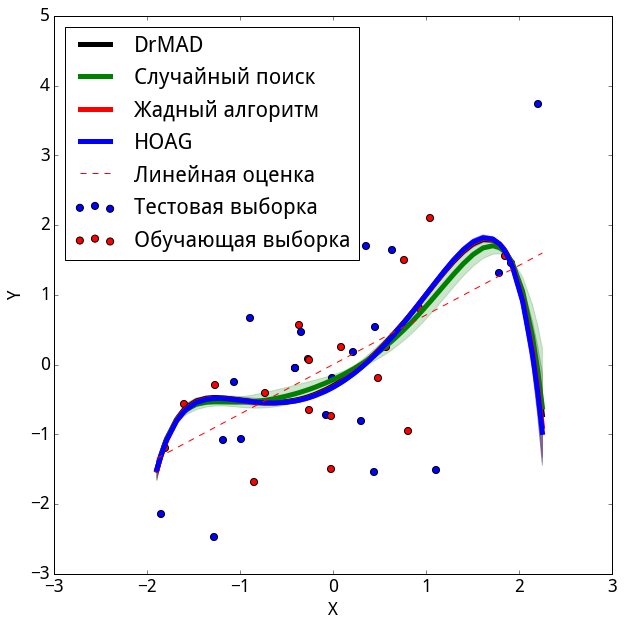
\includegraphics[width=0.8\linewidth]{plots/poly_cv.png}

    \end{subfigure}
    \begin{subfigure}[b]{0.5\textwidth}
    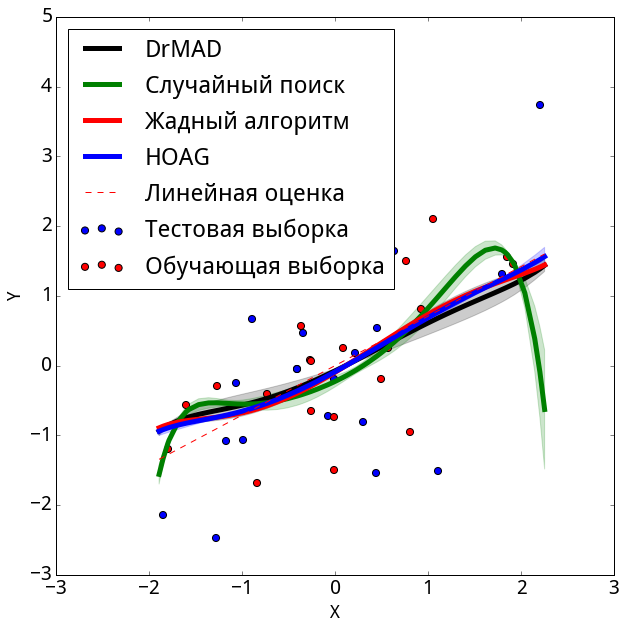
\includegraphics[width=0.8\linewidth]{plots/poly_var.png}

    \end{subfigure}

  \label{fig:poly}
    \caption{Графики итоговых полиномов для синтетической выборки: а --- кросс-валидация, b --- вариационная оценка}
    \end{figure}




    \begin{figure}

    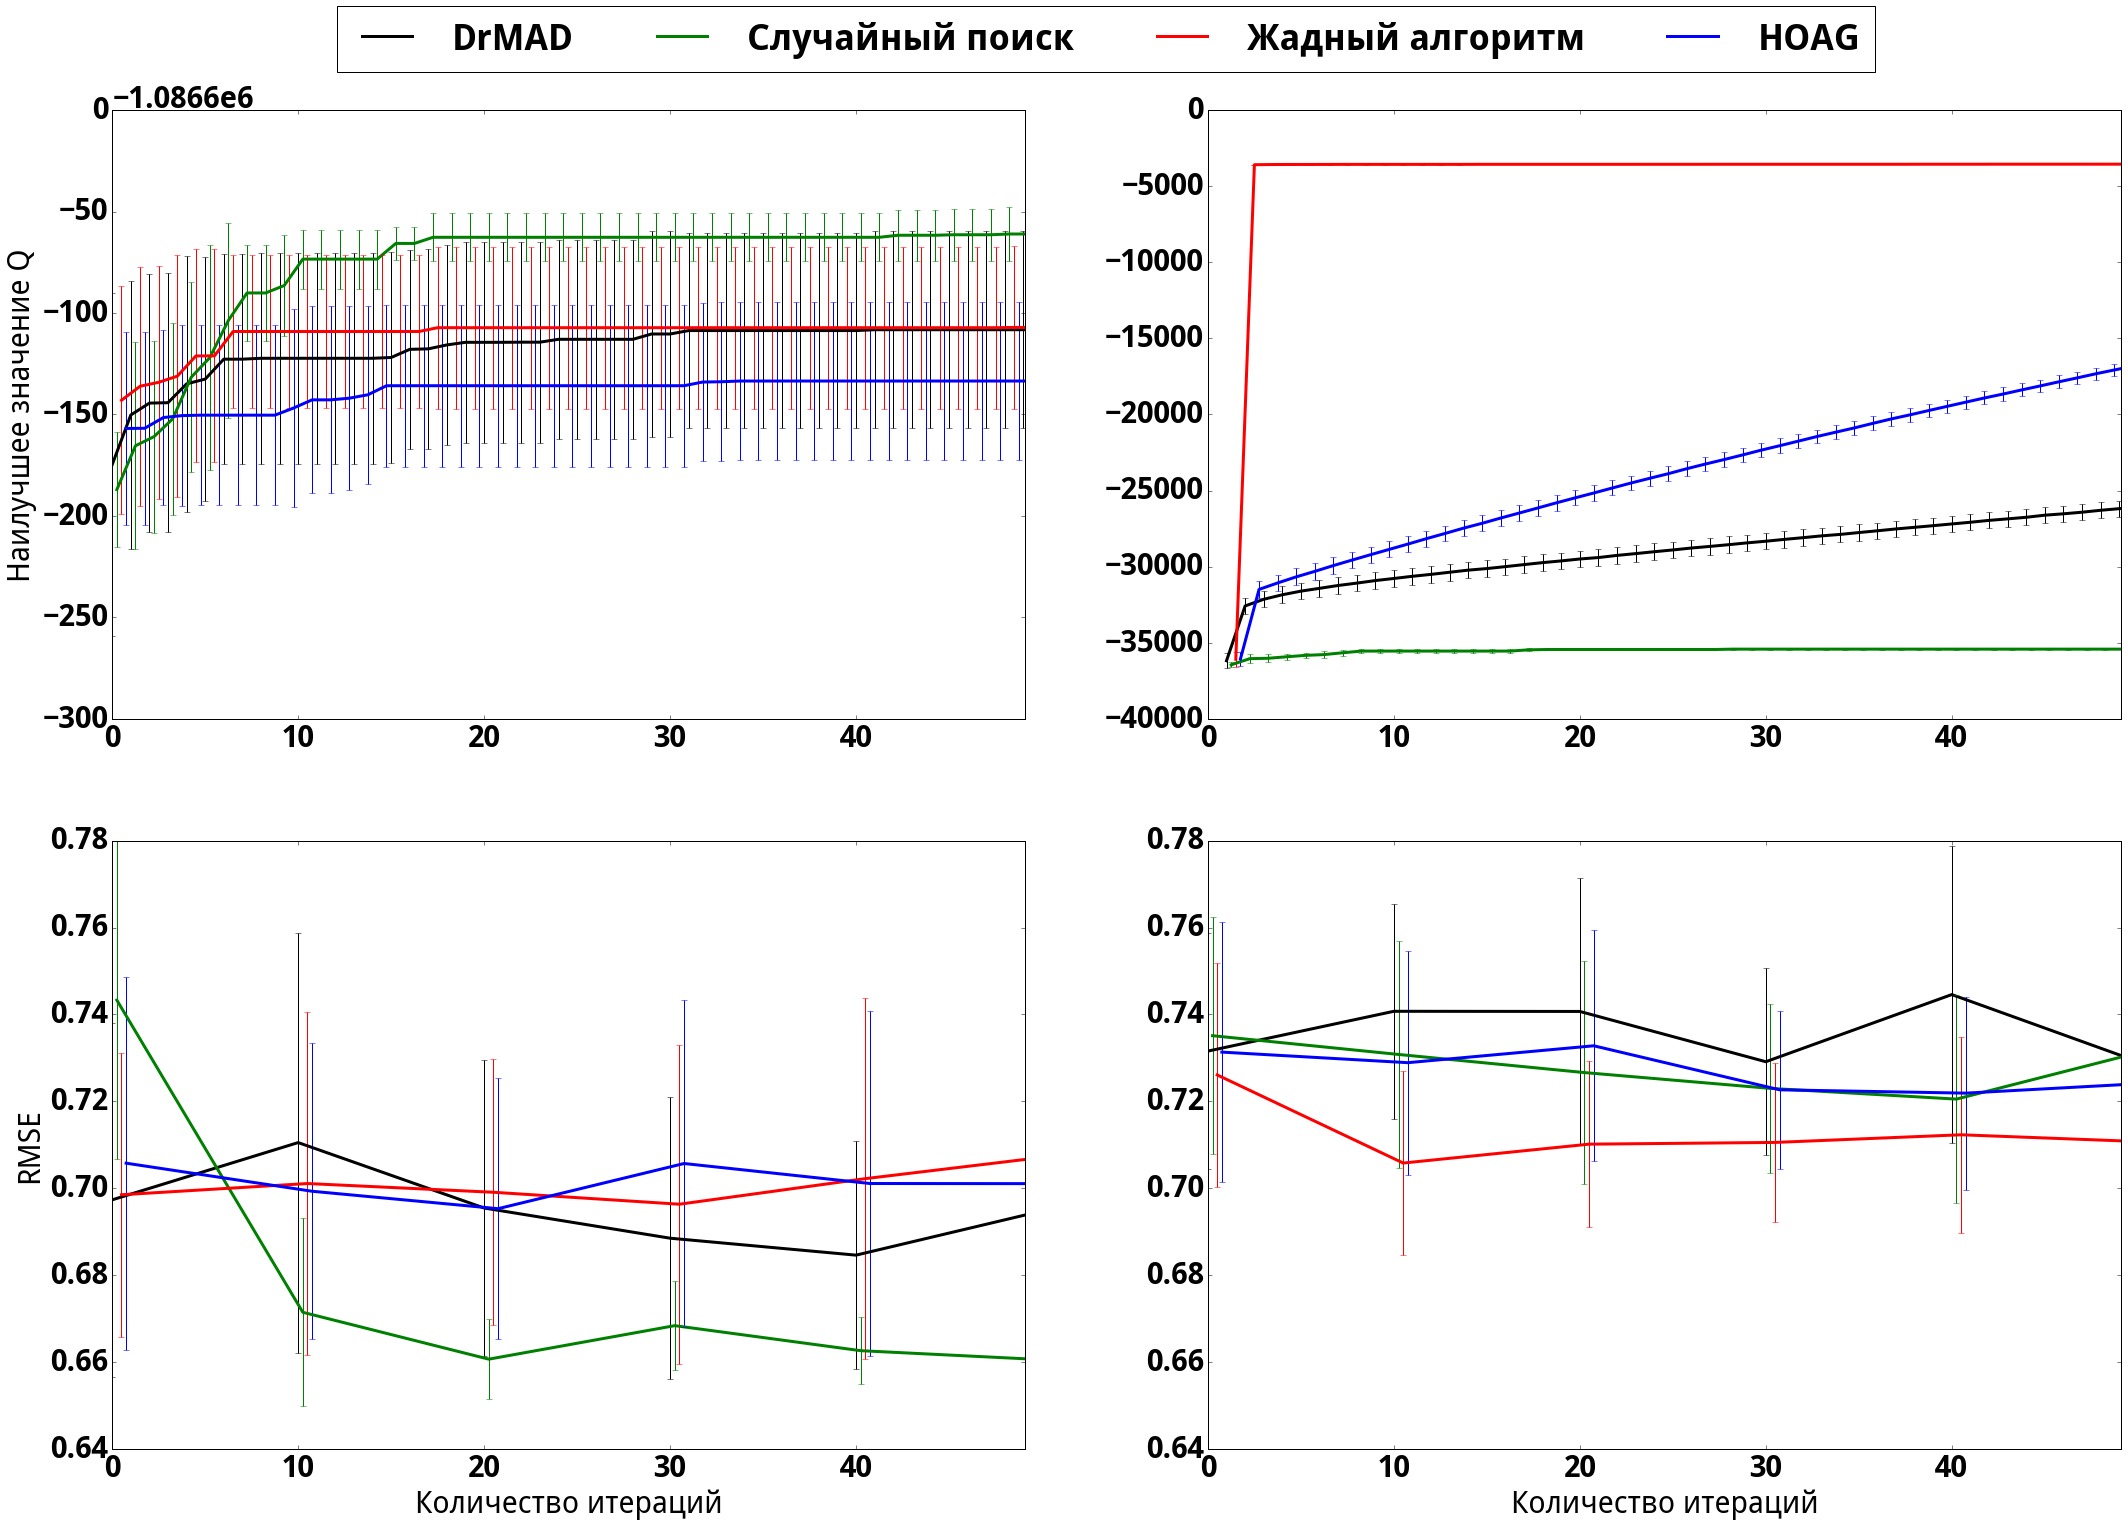
\includegraphics[width=\linewidth]{plots/wisdm.png}

    \caption{Графики завивисимости функции $\hat{Q}$ и качества модели от количества итераций оптимизации для кросс-валидации:  кросс-валидация (слева), вариационная оценка (справа)}
    \end{figure}




\section{Discussion}
\begin{itemize}
\item HOAG и жадный работаю приблизительно одинаково
\item Несмотря на близкую ассимптотику, HOAG предпочтитетелен, если сама внутренняя оптимизация является дорогой
\item С другой стороны - HOAG требует мета-настройки, а жадный алгоритм можно использовать по расписанию
\item DrMAD показывает неустойчивые результаты. 
\item Возможны два улучшения: использование хорошего оптимизатора вместо GD и установка более сложной траектории
\item В отличие от HOAG и жадного, для DrMAD есть предпосылки для оптимизации параметров оптимизации
\end{itemize}
\section{Заключение}
В работе было проведено сравнение градиентных методов оптимизации гиперпараметров.  В качестве базового алгоритма выступал выбор гиперпараметров модели с использованием случайного поиска. В качестве критерия выбора модели выступали вариационная нижняя оценка правдоподобия модели и ошибка на валидационной части выборки, исследованы их свойства и устойчивость получаемых моделей. Было проведено исследование поведения алгоритмов на выборках WISDM и MNIST. В дальнейшем планируется обобщение рассматриваемых методов для проведения мета-оптимизации и получения оценок параметров градиентных оптимизаций.


\addcontentsline{toc}{section}{Список литературы}
\bibliographystyle{utf8gost71u}
%\bibliographystyle{unsrt}
\bibliography{lit}

\end{document}
